\documentclass[preprint,12pt,aps,pra,showkeys,amsmath,amssymb,superscriptaddress,floatfix]{revtex4-2}
\usepackage[T1]{fontenc}
\usepackage[utf8]{inputenc}
\usepackage{amsmath,amssymb,amsthm,mathtools,mathrsfs}
\usepackage{microtype,booktabs,enumitem}
\usepackage{xcolor,tikz,etoolbox}
\usepackage[skins,breakable]{tcolorbox}
\usepackage{needspace}
% Keep diagram geometry independent of REVTeX preprint body spacing.
\AtBeginEnvironment{tikzpicture}{\linespread{1}\selectfont}
\usetikzlibrary{arrows.meta,positioning,calc,fit,decorations.pathreplacing}
\usepackage{graphicx}
\usepackage{hyperref}

\definecolor{MMBlue}{RGB}{0,82,155}
\definecolor{MMOrange}{RGB}{200,80,0}
\tikzset{
 mmnode/.style={draw=MMBlue,rounded corners=2pt,fill=MMBlue!4,align=left,execute at begin node={\raggedright},text width=5cm,font=\fontsize{10}{12}\selectfont,inner sep=6pt},
 mmimport/.style={mmnode,draw=black!65,fill=black!4},
 mmcandidate/.style={mmnode,draw=MMOrange,dashed,fill=MMOrange!5},
 mmrejected/.style={mmnode,draw=black,densely dotted,fill=black!8},
 mmproof/.style={->,thick,MMBlue},
 mmflow/.style={->,semithick,black!70},
 mmrepair/.style={->,dashed,thick,MMOrange},
 mmcandidatearrow/.style={->,dashed,semithick,MMOrange},
 mmnote/.style={font=\scriptsize,fill=white,inner sep=2pt,align=center}}

\usepackage[section]{placeins}
\setlength{\emergencystretch}{3em}
\setlist{itemsep=3pt,topsep=4pt}
\newtheorem{theorem}{Theorem}[section]
\newtheorem{proposition}[theorem]{Proposition}
\newtheorem{lemma}[theorem]{Lemma}
\newtheorem{corollary}[theorem]{Corollary}
\theoremstyle{definition}
\newtheorem{definition}[theorem]{Definition}
\newtheorem{example}[theorem]{Example}
\theoremstyle{remark}
\newtheorem{remark}[theorem]{Remark}
% Avoid isolated statement headings and single-line paragraph fragments.
\BeforeBeginEnvironment{theorem}{\Needspace{6\baselineskip}}
\BeforeBeginEnvironment{definition}{\Needspace{5\baselineskip}}
\BeforeBeginEnvironment{proposition}{\Needspace{5\baselineskip}}
\BeforeBeginEnvironment{lemma}{\Needspace{5\baselineskip}}
\BeforeBeginEnvironment{corollary}{\Needspace{5\baselineskip}}
\clubpenalty=5000
\widowpenalty=5000
\newcommand{\R}{\mathbb R}\newcommand{\Z}{\mathbb Z}\newcommand{\N}{\mathbb N}
\newcommand{\Pa}{\operatorname{Pa}}\newcommand{\Desc}{\operatorname{Desc}}
\newcommand{\cl}{\operatorname{cl}}\newcommand{\cost}{\operatorname{cost}}
\newcommand{\status}{\operatorname{status}}
% Faculty cards: a visual rail groups the five faculties within one agent.
% The rail has no arrowhead and does not represent a proof dependency.
\newcommand{\mmfacultybadge}[1]{%
 \node[circle,draw=MMBlue,line width=1pt,fill=white,
 minimum size=7mm,inner sep=0pt,font=\sffamily\small\bfseries,text=MMBlue]
 at ([xshift=15pt,yshift=-15pt]frame.north west) {#1};}
\newcommand{\mmfacultyrail}{%
 \draw[MMBlue!80,line width=1pt]
 ([xshift=15pt,yshift=2pt]frame.north west)--
 ([xshift=15pt,yshift=-2pt]frame.south west);}
\newtcolorbox{mmfacultybox}[2]{enhanced,breakable,
 colback=MMBlue!4,colframe=MMBlue!4,boxrule=0pt,arc=3pt,
 left=39pt,right=9pt,top=4pt,bottom=4pt,
 before skip=2pt,after skip=2pt,
 fontupper=\small\linespread{1.1}\selectfont,
 overlay unbroken={\mmfacultyrail\mmfacultybadge{#1}},
 overlay first={\mmfacultyrail\mmfacultybadge{#1}},
 overlay middle={\mmfacultyrail},overlay last={\mmfacultyrail}}
\newcommand{\mmfaculty}[3]{%
 \begin{mmfacultybox}{#1}{#2}
 {\sffamily\bfseries\color{MMBlue}#2}\par\smallskip #3
 \end{mmfacultybox}}
\newcommand{\agent}[9]{%
 \Needspace{8\baselineskip}
 \subsubsection{#1}
 \noindent\textbf{Object.} #2\par
 \noindent\textbf{Role.} #3\par\smallskip
 \mmfaculty{E}{Ego}{#4}
 \mmfaculty{M}{Memory}{#5}
 \mmfaculty{I}{Intellect}{#6}
 \mmfaculty{S}{Sense}{#7}
 \mmfaculty{A}{Action}{#8}
 \smallskip\noindent #9\par}

\usepackage{longtable,array,calc}
\providecommand{\tightlist}{\setlength{\itemsep}{2pt}\setlength{\parskip}{0pt}}
\makeatletter
\def\frontmatter@abstract@produce{\par\addvspace{\frontmatter@preabstractspace}%
\begingroup\prep@absbox\unvbox\absbox\post@absbox\endgroup
\addvspace{\frontmatter@postabstractspace}}
\makeatother
\newcommand{\field}[2]{\par\smallskip\noindent\textbf{#1.} #2\par}
\setlength{\emergencystretch}{5em}
\AtBeginEnvironment{verbatim}{\small\linespread{1.0}\selectfont}


\hypersetup{colorlinks=true,linkcolor=MMBlue,urlcolor=MMBlue,pdfauthor={Dibakar Sigdel}}

\begin{document}

\title{Hahn--Banach Norm-Preserving Extension\\[4pt]\large An End-to-End Meta-Math Walkthrough}

\author{Dibakar Sigdel}

\affiliation{Mindverse Computing LLC, Lynnwood, WA 98087, USA}

\date{October 2026}

\begin{abstract}

The key finite step extends a dominated functional by one direction. A
chain-union argument then extends it to the entire space without
claiming countably many directions suffice. The report presents the
target theorem, declared imports, a dependency graph, five-faculty node
contracts, a continuous proof, a worked example, and a hypothesis-repair
audit. It is an authored mathematical exposition, not a deployed-agent
transcript or a formal proof-assistant certificate.

\end{abstract}\maketitle\linespread{1.12}\selectfont

\noindent\textbf{FA-05 / Functional Analysis and Measure Theory / Report v1}

\section{Target and import contract}

\begin{theorem}

Let \(X\) be a real normed space, \(M\subset X\) any linear subspace,
and \(f:M\to\mathbb R\) bounded linear. There exists bounded linear
\(F:X\to\mathbb R\) with \(F|_M=f\) and \(\|F\|=\|f\|\). Neither
completeness of \(X\) nor closedness of \(M\) is assumed.

\end{theorem}

\subsection{Foundations and permitted imports}

Work in set theory with Zorn's lemma: a nonempty partially ordered set
in which every chain has an upper bound has a maximal element. Let
\(C=\|f\|\) and \(p(x)=C\|x\|\), a finite-valued sublinear function:
\(p(x+y)\le p(x)+p(y)\) and \(p(tx)=tp(x)\) for \(t\ge0\). Use
completeness of the real order to select a number between a bounded
supremum and infimum.

\clearpage\section{Node interaction workflow}

\begin{center}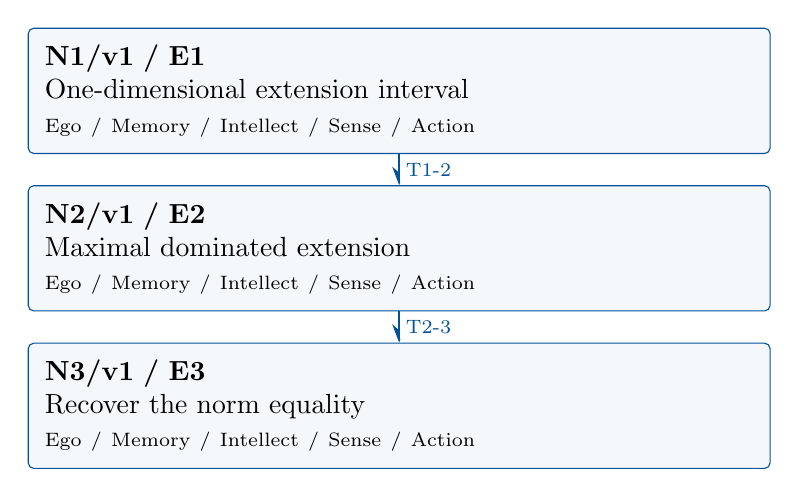
\begin{tikzpicture}[>=Stealth,x=1cm,y=1cm]

\node[mmnode,text width=9cm,minimum height=1.25cm] (N1) at (0,0.0) {\textbf{N1/v1 / E1}\\One-dimensional extension interval\\{\scriptsize Ego / Memory / Intellect / Sense / Action}};

\node[mmnode,text width=9cm,minimum height=1.25cm] (N2) at (0,-2.0) {\textbf{N2/v1 / E2}\\Maximal dominated extension\\{\scriptsize Ego / Memory / Intellect / Sense / Action}};

\node[mmnode,text width=9cm,minimum height=1.25cm] (N3) at (0,-4.0) {\textbf{N3/v1 / E3}\\Recover the norm equality\\{\scriptsize Ego / Memory / Intellect / Sense / Action}};

\draw[mmproof] (N1.south) -- node[mmnote,right] {T1-2} (N2.north);

\draw[mmproof] (N2.south) -- node[mmnote,right] {T2-3} (N3.north);

\end{tikzpicture}\end{center}

Each box is one mathematical agent containing all five faculties. Blue
arrows carry the versioned exports listed below. The layout gives a
reading order; only drawn arrows assert dependencies. Diagnostic repair
is separate from the proof DAG.

\subsection{Versioned evidence-transfer ledger}

\begingroup\small\linespread{1.05}\selectfont

\Needspace{5\baselineskip}\field{T1-2: N1/E1/v1 to N2}{\(g\) extends linearly to \(D+\mathbb Rz\) while remaining dominated by
\(p\).}

\field{Receiving activity}{N2.2}

\field{Compatibility}{E1/v1 and all extensions of \(f\) dominated by \(p\). Check: A union is
a function only because the extensions agree on overlaps; a maximal
proper domain can still be extended by E1.}

\Needspace{5\baselineskip}\field{T2-3: N2/E2/v1 to N3}{There is a linear \(F:X\to\mathbb R\) extending \(f\) with \(F\le p\).}

\field{Receiving activity}{N3.1}

\field{Compatibility}{E2/v1 and \(p(x)=C\|x\|\). Check: One-sided domination alone must be
converted to an absolute bound; the zero-functional case is included.}

\endgroup

\clearpage\section{Agent roles and five-faculty activities}\begingroup\small\linespread{1.05}\selectfont\setlist{itemsep=1pt,topsep=2pt}

\begingroup\footnotesize\linespread{1.05}\selectfont\let\small\footnotesize

\subsection{N1/v1: One-dimensional extension interval}

\field{Object and role}{Turn domination of \(g(d)+ta\) into compatible lower and upper bounds
for the new value \(a=G(z)\). \textbf{Local obligation:} \(g\) extends
linearly to \(D+\mathbb Rz\) while remaining dominated by \(p\).}

\field{Inputs}{A linear \(g:D\to\mathbb R\) with \(g\le p\) on a subspace \(D\), and
\(z\notin D\).}

\mmfaculty{E}{Ego}{Publish E1/v1 only after establishing this obligation: \(g\) extends
linearly to \(D+\mathbb Rz\) while remaining dominated by \(p\).}

\mmfaculty{M}{Memory}{A linear \(g:D\to\mathbb R\) with \(g\le p\) on a subspace \(D\), and
\(z\notin D\). Retain the stated assumptions and import versions.}

\mmfaculty{I}{Intellect}{Turn domination of \(g(d)+ta\) into compatible lower and upper bounds
for the new value \(a=G(z)\).}

\mmfaculty{S}{Sense}{Both signs of \(t\) must be checked, and the choice interval must be
nonempty and finite.}

\mmfaculty{A}{Action}{Carry out activities N1.1--N1.3 below, retaining each calculation and
construction as evidence.}

\smallskip\noindent\textbf{Numbered mathematical activities}

\begin{enumerate}[label=N1.\arabic*,leftmargin=3.4em]

\item For \(u,v\in D\), linearity and domination give
\(g(u)+g(v)=g(u+v)\le p(u+v)\le p(u-z)+p(v+z)\). Therefore
\(g(u)-p(u-z)\le p(v+z)-g(v)\). Set \(L=\sup_u[g(u)-p(u-z)]\) and
\(U=\inf_v[p(v+z)-g(v)]\). The preceding inequality gives \(L\le U\);
choosing \(u=0\) and \(v=0\) bounds both endpoints between finite
numbers.

\item Choose \(a\in[L,U]\) and define \(G(d+tz)=g(d)+ta\). The representation
is unique because \(z\notin D\), so \(G\) is well defined and linear.
For \(t>0\), \(a\le p(d/t+z)-g(d/t)\) implies \(G(d+tz)\le p(d+tz)\).

\item For \(t=-s<0\), \(a\ge g(d/s)-p(d/s-z)\) gives
\(g(d)-sa\le s p(d/s-z)=p(d-sz)\). The case \(t=0\) uses \(g\le p\).
Thus domination holds for every real scalar.

\end{enumerate}

\field{Export E1/v1}{\(g\) extends linearly to \(D+\mathbb Rz\) while remaining dominated by
\(p\).}

\field{Acceptance gate}{Both signs of \(t\) must be checked, and the choice interval must be
nonempty and finite.}

\field{Targeted repair}{If only positive scalars were considered, restore the lower endpoint
\(L\) and the negative-scalar calculation before extending the domain.
Withhold this export and recheck its descendants after a versioned
correction.}

\endgroup

\clearpage

\subsection{N2/v1: Maximal dominated extension}

\field{Object and role}{Order compatible extensions by domain inclusion and take unions along
chains. \textbf{Local obligation:} There is a linear \(F:X\to\mathbb R\)
extending \(f\) with \(F\le p\).}

\field{Inputs}{E1/v1 and all extensions of \(f\) dominated by \(p\). Incoming proof
exports: E1/v1 at N2.2.}

\mmfaculty{E}{Ego}{Publish E2/v1 only after establishing this obligation: There is a linear
\(F:X\to\mathbb R\) extending \(f\) with \(F\le p\).}

\mmfaculty{M}{Memory}{E1/v1 and all extensions of \(f\) dominated by \(p\). Incoming proof
exports: E1/v1 at N2.2. Retain the stated assumptions and import
versions.}

\mmfaculty{I}{Intellect}{Order compatible extensions by domain inclusion and take unions along
chains.}

\mmfaculty{S}{Sense}{A union is a function only because the extensions agree on overlaps; a
maximal proper domain can still be extended by E1.}

\mmfaculty{A}{Action}{Carry out activities N2.1--N2.2 below, retaining each calculation and
construction as evidence.}

\smallskip\noindent\textbf{Numbered mathematical activities}

\begin{enumerate}[label=N2.\arabic*,leftmargin=3.4em]

\item The set of pairs \((D,g)\) with \(M\subset D\subset X\), \(g|_M=f\), and
\(g\le p\) is nonempty. Order it by extension. For a chain, the union of
its domains is a subspace: any two vectors and their values occur
together in one chain member. The union map is consequently well
defined, linear, and dominated by \(p\).

\item This union is an upper bound, so Zorn supplies a maximal pair \((D,g)\).
If \(D\ne X\), choose \(z\in X\setminus D\) and apply E1, contradicting
maximality. Thus \(D=X\); denote the resulting map by \(F\).

\end{enumerate}

\field{Export E2/v1}{There is a linear \(F:X\to\mathbb R\) extending \(f\) with \(F\le p\).}

\field{Acceptance gate}{A union is a function only because the extensions agree on overlaps; a
maximal proper domain can still be extended by E1.}

\field{Targeted repair}{If a union of incomparable extensions is used, restrict to chains before
invoking Zorn; arbitrary extensions can assign conflicting values.
Withhold this export and recheck its descendants after a versioned
correction.}

\clearpage

\subsection{N3/v1: Recover the norm equality}

\field{Object and role}{Apply the one-sided domination to \(x\) and \(-x\), then compare with
the restriction. \textbf{Local obligation:} \(F|_M=f\) and
\(\|F\|=\|f\|\).}

\field{Inputs}{E2/v1 and \(p(x)=C\|x\|\). Incoming proof exports: E2/v1 at N3.1.}

\mmfaculty{E}{Ego}{Publish E3/v1 only after establishing this obligation: \(F|_M=f\) and
\(\|F\|=\|f\|\).}

\mmfaculty{M}{Memory}{E2/v1 and \(p(x)=C\|x\|\). Incoming proof exports: E2/v1 at N3.1. Retain
the stated assumptions and import versions.}

\mmfaculty{I}{Intellect}{Apply the one-sided domination to \(x\) and \(-x\), then compare with
the restriction.}

\mmfaculty{S}{Sense}{One-sided domination alone must be converted to an absolute bound; the
zero-functional case is included.}

\mmfaculty{A}{Action}{Carry out activities N3.1--N3.2 below, retaining each calculation and
construction as evidence.}

\smallskip\noindent\textbf{Numbered mathematical activities}

\begin{enumerate}[label=N3.\arabic*,leftmargin=3.4em]

\item For every \(x\), \(F(x)\le C\|x\|\) and \(-F(x)=F(-x)\le C\|x\|\). Hence
\(|F(x)|\le C\|x\|\), so \(F\) is bounded and \(\|F\|\le C\).

\item Restricting \(F\) to the unit ball of \(M\) gives \(\|f\|\le\|F\|\).
Since \(C=\|f\|\), equality follows. If \(C=0\), this argument yields
\(F=0\) and still applies.

\end{enumerate}

\field{Export E3/v1}{\(F|_M=f\) and \(\|F\|=\|f\|\).}

\field{Acceptance gate}{One-sided domination alone must be converted to an absolute bound; the
zero-functional case is included.}

\field{Targeted repair}{If the norm conclusion is inferred directly from \(F\le p\), add the
\(-x\) bound and the restriction inequality. Withhold this export and
recheck its descendants after a versioned correction.}

\endgroup\clearpage\section{Continuous mathematical proof}\label{sec:proof}

\subsection{N1 --- One-dimensional extension
interval}\label{n1-one-dimensional-extension-interval}

\begin{enumerate}
\def\labelenumi{\arabic{enumi}.}
\item
  \textbf{N1.1.} For \(u,v\in D\), linearity and domination give
  \(g(u)+g(v)=g(u+v)\le p(u+v)\le p(u-z)+p(v+z)\). Therefore
  \(g(u)-p(u-z)\le p(v+z)-g(v)\). Set \(L=\sup_u[g(u)-p(u-z)]\) and
  \(U=\inf_v[p(v+z)-g(v)]\). The preceding inequality gives \(L\le U\);
  choosing \(u=0\) and \(v=0\) bounds both endpoints between finite
  numbers.
\item
  \textbf{N1.2.} Choose \(a\in[L,U]\) and define \(G(d+tz)=g(d)+ta\).
  The representation is unique because \(z\notin D\), so \(G\) is well
  defined and linear. For \(t>0\), \(a\le p(d/t+z)-g(d/t)\) implies
  \(G(d+tz)\le p(d+tz)\).
\item
  \textbf{N1.3.} For \(t=-s<0\), \(a\ge g(d/s)-p(d/s-z)\) gives
  \(g(d)-sa\le s p(d/s-z)=p(d-sz)\). The case \(t=0\) uses \(g\le p\).
  Thus domination holds for every real scalar.
\end{enumerate}

\subsection{N2 --- Maximal dominated
extension}\label{n2-maximal-dominated-extension}

\begin{enumerate}
\def\labelenumi{\arabic{enumi}.}
\item
  \textbf{N2.1.} The set of pairs \((D,g)\) with
  \(M\subset D\subset X\), \(g|_M=f\), and \(g\le p\) is nonempty. Order
  it by extension. For a chain, the union of its domains is a subspace:
  any two vectors and their values occur together in one chain member.
  The union map is consequently well defined, linear, and dominated by
  \(p\).
\item
  \textbf{N2.2.} This union is an upper bound, so Zorn supplies a
  maximal pair \((D,g)\). If \(D\ne X\), choose \(z\in X\setminus D\)
  and apply E1, contradicting maximality. Thus \(D=X\); denote the
  resulting map by \(F\).
\end{enumerate}

\subsection{N3 --- Recover the norm
equality}\label{n3-recover-the-norm-equality}

\begin{enumerate}
\def\labelenumi{\arabic{enumi}.}
\item
  \textbf{N3.1.} For every \(x\), \(F(x)\le C\|x\|\) and
  \(-F(x)=F(-x)\le C\|x\|\). Hence \(|F(x)|\le C\|x\|\), so \(F\) is
  bounded and \(\|F\|\le C\).
\item
  \textbf{N3.2.} Restricting \(F\) to the unit ball of \(M\) gives
  \(\|f\|\le\|F\|\). Since \(C=\|f\|\), equality follows. If \(C=0\),
  this argument yields \(F=0\) and still applies.
\end{enumerate}

\hfill$\square$

\section{Worked orchestration}

In \(\mathbb R^2\) with the Euclidean norm, take \(M=\{(t,t)\}\) and
\(f(t,t)=2t\). The norm on \(M\) is \(\sqrt2\). The extension
\(F(x,y)=x+y\) has norm \(\sqrt2\) and restricts correctly. This is a
concrete certificate; the general construction does not promise a unique
extension.

\subsection{Boundary and hypothesis audit}

Uniqueness is false. In \(\mathbb R^2\) with the \(\ell^1\) norm, let
\(M\) be the first coordinate axis and \(f(x,0)=x\). Every
\(F_a(x,y)=x+ay\) with \(|a|\le1\) extends \(f\) and has norm one.

\section{Illustrative failure and repair}

The following is an authored diagnostic scenario. Changed assumptions
define a new contract; they do not retroactively prove the original
statement.

\subsection{Rejected argument, diagnosis, and correction}
\textbf{Rejected N1 candidate:} choose any \(a\) below the upper bound
and ignore the lower bound. For \(X=\mathbb R\), \(D=\{0\}\),
\(p(t)=|t|\), choosing \(a=-2\) satisfies \(a\le1\) but fails domination
at \(-1\), where \(G(-1)=2>1\). \textbf{Repair:} require \(a\in[-1,1]\),
the actual two-sided interval. This corrects the extension argument
under the same theorem. Recheck the maximal-extension and norm exports.

\subsection{Publication and reuse}
The corrected export retains its explicit assumptions. A hypothetical
revision receives a new version, and each consuming activity is
rechecked; this scenario is not a recorded runtime event. \textbf{Next
direction:} Deduce that every nonzero vector has a norming continuous
linear functional by first defining it on its one-dimensional span.

\par\medskip\begingroup\small\linespread{1.0}\selectfont\noindent\textbf{Provenance.} This authored proof is complete relative to its declared imports. Reuse
each export with its assumptions, proof, and version. The original
Markdown remains available for comparison.
\par\endgroup

\par\smallskip\begingroup\small\linespread{1.0}\selectfont\noindent\textbf{Further reading.} \href{https://ocw.mit.edu/courses/18-102-introduction-to-functional-analysis-spring-2021/resources/lecture-notes/}{MIT
OpenCourseWare, Introduction to Functional Analysis: lecture notes}. See
the lectures on integration, Hilbert spaces, Baire category, and
Hahn--Banach.\par\endgroup

\end{document}
